\documentclass[../main/main.tex]{subfiles}
\begin{document}

\dominitoc
\faketableofcontents
\dominilof
\fakelistoffigures
\dominilot
\fakelistoftables

\chapter{Perspectives et discussion}\label{ch:persp}
\epigraph{\openquote\textit{A common mistake that people make when trying to
design something completely foolproof is to underestimate the ingenuity of
complete fools}\closequote}{Douglas \textsc{Adams}, \textit{Mostly Harmless}}

Au travers de cette thèse, nous avons utilisé un certain lot de données pour
mettre en place un modèle d'évolution de l'étirement des SNe~Ia avec le
redshift. Nous avons pour cela dû effectuer des coupes en redshift afin de
limiter les effets de sélection dans l'échantillon, amenant notre nombre total
de SNe~Ia à 569. Ce modèle a permis de donner des premières indications fortes
sur le fait que les propriétés des SNe~Ia dérivent avec le redshift, établissant
que tout modèle non-dérivant ne saurait décrire aussi bien les données que celui
proposé. Nous avons ensuite implémenté ce modèle ainsi que la marche de
magnitude basée sur l'âge dans l'outil de simulation et d'analyses cosmologiques
\snana. Cette étude nous a permis de tester les biais potentiels sur le calcul
du paramètre cosmologique $w$, que l'on trouve autour de 4\%.

Depuis la première partie de cette étude, de nouvelles données sont cependant
disponibles grâce aux travaux d'envergure menés par la \textit{Zwicky Transient
Facility} \citep[ZTF,][]{bellm2019}. Elles s'avèrent particulièrement utile par
leur localisation autour de $z \lesssim 0,1$~; nous proposons
Section~\ref{sec:xztf} de les inclure à notre analyse première afin de raffiner
le modèle.

Les simulations effectuées avec \snana\ se sont vues limitées par le temps de
calcul et la complexité de la prise en main des logiciels. Nous proposons
Section~\ref{sec:simpersp} des pistes d'amélioration en vue de continuer cette
étude et ouvrir la voix à l'implémentation complète de l'âge dans cet outil.

\vfill
\minitoc
\vfill

\newpage

\section{Étirement~: inclusion des données de ZTF}\label{sec:xztf}

Dans le Chapitre~\ref{ch:stretch}, nous avions considéré une modélisation simple
par mélange Gaussien à deux populations. Des données supplémentaires exemptes de
biais de \textsc{Malmquist} significatifs nous permettraient de l'affiner.
Notamment, les données aux extrémités à bas et haut redshifts du diagramme de
\textsc{Hubble} sont particulièrement utiles pour l'analyse de cette dérive. Si
les programmes de relevé de SNe~Ia à haut redshifts Subaru et SeeChange ne sont
pas encore disponibles, les données fournies par la \textit{Zwicky Transient
Facility} \citep[ZTF,][]{bellm2019, graham2019} nous ont permis d'établir un
échantillon extrêmement riche à bas redshift, 2246 SNe~Ia entre $0,0 < z < 0,19$
(voir Chapitre~\ref{ch:surveys}, Tableau~\ref{tab:sondcomp}). L'établissement de
sa partie limitée en volume a été détaillée Chapitre~\ref{ch:sample}, et se
compose de 638 SNe~Ia dans sa partie fiducielle, pour un redshift limite de
0,055.

\subsection{Prédiction}\label{ssec:xpred}

Étant donné la faible valeur de ce redshift moyen, le grand échantillonnage et
sa qualité non-ciblée, nous nous attendons à ce que les données d'étirement de
ce sondage suive la distribution du modèle de référence pris à très bas
redshift. Notamment, ce modèle suppose la présence d'un pic dans la quantité de
données à petit étirement, autour de $x_1 \approx -1,5$ (voir, par exemple, la
courbe jaune de la ligne 2 et colonne 1 de la Figure~\ref{fig:mod_all}). C'est
en effet ce que nous observons dans l'histogramme des données d'étirement de ce
sondage, peu importe la coupe choisie. Nous présentons
Figure~\ref{fig:N21HDZTFerr} l'histogramme des données fiducielles de ZTF sur
lequel nous présentons le modèle de base ajusté sur l'échantillon de base
(modèle ci-après appelé N21) et son erreur.

\begin{SCfigure}[1][ht]
    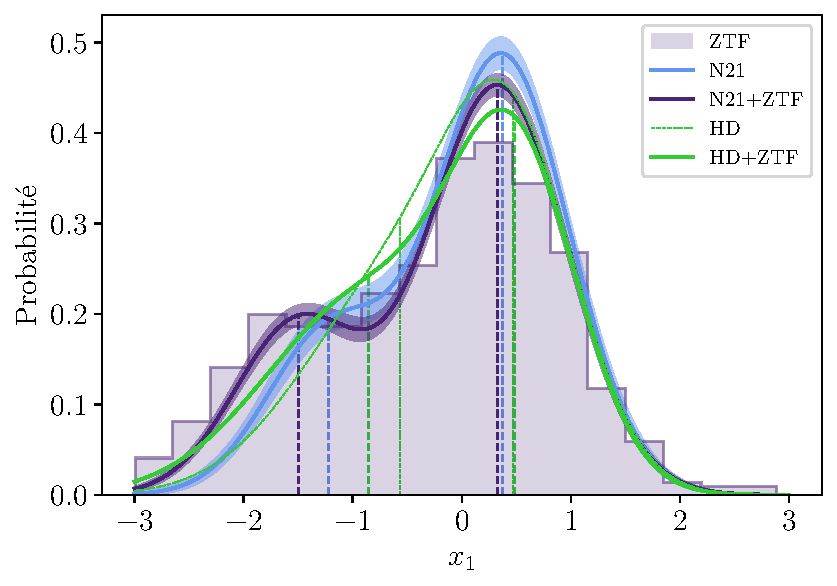
\includegraphics[width=.6\linewidth]{model_N21+HD+ZTF_on_ZTF}
    \caption[Accord entre les modèles N21+ZTF et HD+ZTF et l'histogramme des
    étirements de ZTF]{En violet~: histogramme des étirements de ZTF. En
        bleu (violet) et leurs bandes~: modèles de base ajustés sur
        l'échantillon de base, N21, (échantillon avec ZTF, N21+ZTF) au
        redshift moyen de ZTF et leur erreur. En fin pointillés verts (ligne
        continue)~: modèles Howell+dérive ajustés sur l'échantillon de base,
    HD (échantillon avec ZTF, HD+ZTF).}
    \label{fig:N21HDZTFerr}
\end{SCfigure}

Nous remarquons que s'il existe bien un pic de petit étirement, le modèle N21 ne
saurait le caractériser correctement, la distribution étant trop écartée de ce
que nous pourrions considérer comme la moyenne de ce mode de petit étirement. Il
reste bien plus proche que le modèle Howell+dérive ajusté sur l'échantillon de
base (ci-après HD), représenté en fins pointillés verts
Figure~\ref{fig:N21HDZTFerr}.

\subsection{Implémentation}\label{ssec:xamel}

Nous constatons que même si le sondage SNf a permis l'établissement d'un modèle
robuste \textit{via} l'utilisation du LsSFR comme traceur de l'âge, le manque de
données à bas redshift limite la force de ces résultats. C'est pourquoi nous
proposons d'inclure les données de ZTF dans cette étude. Les résultats de
l'ajustement de ce modèle à l'ensemble des 1207 (respectivement 815) SNe~Ia de
l'échantillon fiduciel+ZTF (conservatif+ZTF) sont présentés dans le
Tableau~\ref{tab:modelresults_ztf}. Comme attendu, les paramètres du mode de
grand étirement $(\mu_1,\sigma_1$) ne diffèrent pas significativement des
résultats précédents, mais la moyenne du mode de petit étirement $\mu_2$ est
bien plus basse et incompatible avec les résultats de base. Nous pouvons
également noter une baisse de l'amplitude du mode 1 dans la combinaison linéaire
composant la distribution sous-jacente de la vieille population, donnant donc
plus d'amplitude au mode de petits étirements.

\begin{table*}
    \centering
        \caption[Valeurs des paramètres du modèle d'étirement de base selon
        l'échantillon avec les données de ZTF]{Valeurs des paramètres issus des
            meilleurs ajustements du modèle de distribution de l'étirement de
            base lorsqu'il est appliqué à l'ensemble de données de base
            seulement (569 SNe~Ia), à l'échantillon fiduciel avec ZTF (1207) ou
        à l'échantillon conservatif avec ZTF (815).}
        \label{tab:modelresults_ztf}
    \begin{threeparttable}
        \makebox[\linewidth]{%
        \begin{tabular}{lccccc}
            \toprule
            Échantillon      & $\mu_1$             & $\sigma_1$
                             & $\mu_2$             & $\sigma_2$
                             & $a$ \\
            \midrule
            Base             & $ 0.37 \pm 0.04$    & $0.61 \pm 0.03$
                             & $-1.22 \pm 0.11$    & $0.56 \pm 0.07$
                             & $ 0.51 \pm 0.07$ \\
            Fiduciel+ZTF     & $ 0.33 \pm 0.03$    & $0.64 \pm 0.02$
                             & $-1.50 \pm 0.06$    & $0.58 \pm 0.04$
                             & $ 0.45 \pm 0.04$ \\
            Conservatif+ZTF  & $ 0.35 \pm 0.03$    & $0.61 \pm 0.02$
                             & $-1.50 \pm 0.06$    & $0.54 \pm 0.04$
                             & $ 0.45 \pm 0.04$ \\
            \bottomrule
    \end{tabular}}
        \begin{tablenotes}[flushleft]
            \item\small \textbf{\hspace{-3.2pt}Notes.} La différence principale se
                situe sur la position de la moyenne du mode de bas étirement,
                $\mu_2$, complètement incompatible avec la moyenne résultant de
                l'ajustement avec les données de base~; nous notons également
                l'augmentation de l'amplitude de ce mode \textit{via} la
                réduction du paramètre $a$ décrivant l'amplitude relative des
                deux modes dans la distribution sous-jacente de la population
                vieille.
        \end{tablenotes}
    \end{threeparttable}
\end{table*}

Le modèle de base ajusté sur l'échantillon incluant les données de ZTF est
ci-après nommé N21+ZTF, de même pour le modèle Howell+dérive qui sera nommé
HD+ZTF. Nous donnons Figure~\ref{fig:N21HDZTFerr} les représentations graphiques
de ces quatre distributions au redshift moyen des données de ZTF. Nous
constatons que le modèle N21+ZTF possède alors un second pic de bas étirements
plus éloigné en moyenne que le modèle N21, donnant un meilleur ajustement quand
nous le comparons à l'histogramme des étirements de ZTF, comme attendu. Le modèle
HD+ZTF bénéficie aussi de l'inclusion de ces données, sa moyenne de petits
étirements étant plus proche de la valeur centrale de ce pic~; elle reste
cependant toujours plus éloignée que celle définie par le modèle N21. Les
évolutions prédites de l'étirement avec le redshift ($x_1$ attendu compte tenu
de la distribution de l'équation~\ref{eq:stretchz}) sont illustrées sous la
forme d'une bande violette pour N21+ZTF et bleue pour N21 dans la
Figure~\ref{fig:evol_all_ztf}, qui tiennent compte des erreurs des paramètres et
de leurs covariances. Cette figure montre que l'étirement moyen mesuré des
SNe~Ia par intervalle de redshift (contenant tous le même nombre de données
selon l'échantillon utilisé pour l'ajustement) suit de près notre modélisation
de la dérive avec le redshift~; cependant les deux modèles N21 et N21+ZTF ne
sont pas compatibles entre eux. Nous avons également représenté les évolutions
des modèles HD et HD+ZTF en vert pointillé et plein respectivement. Alors que
dans la Figure~\ref{fig:N21HDZTFerr} la moyenne du mode de petit étirement de
HD+ZTF se rapproche plus du pic de la distribution de ZTF que celle de HD, il
s'écarte beaucoup plus du modèle de base ajusté sur l'échantillon combiné que ce
dernier. Alors que dans N21, ce modèle était relativement compatible avec le
modèle de référence, l'ajout des données de ZTF le rend incompatible avec le
modèle de base. 

\begin{figure}[ht]
    \centering
    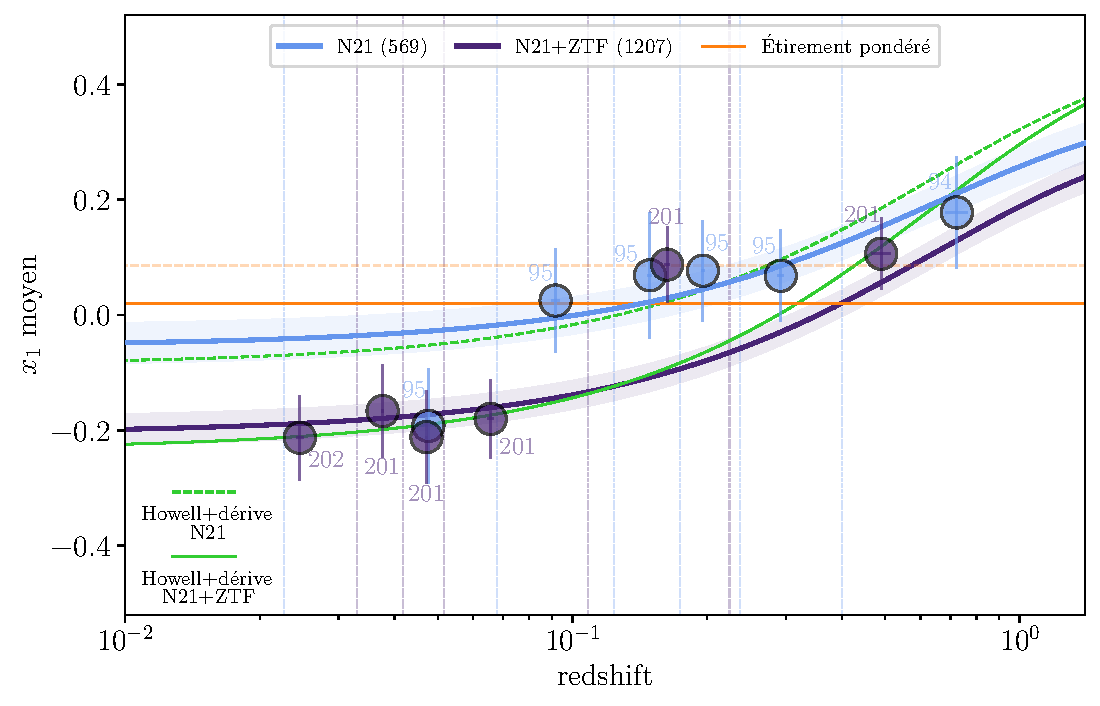
\includegraphics[width=1\linewidth]{stretchevol_all-oth_vs_ztf-weighted.pdf}
    \caption[Évolution de l'étirement moyen des SNe~Ia en fonction du redshift
    issu de la prédiction de notre modèle de base selon l'échantillon
    utilisé]{\footnotesize En bleu (et sa bande)~: évolution de l'étirement
        moyen ($x_1$) des SNe~Ia issus d'un ajustement \texttt{SALT2.4} en
        fonction du redshift pour notre modèle de base ajusté sur les données de
        base, nommé N21 (et son erreur). En violet (et sa bande)~: même modèle
        mais ajusté sur les données de base combinées aux données de ZTF, nommé
        N21+ZTF (et son erreur). Ces deux modèles ne sont pas compatibles entre
        eux. Les marqueurs montrent la moyenne pondérée de l'étirement mesurée
        dans des intervalles de redshift de tailles d'échantillon égales pour
        chaque ensemble de données, indiquées en bleu clair et en violet clair à
        côté de chaque point de mesure pour les modèles N21 et N21+ZTF,
        respectivement. La ligne horizontale orange pleine (pointillée)
        représente l'étirement pondéré des données. La ligne verte (pointillée)
        représente le meilleur ajustement du modèle Howell+dérive ajusté sur
        l'échantillon fiduciel combiné à ZTF (fiduciel de base). Alors que dans
        N21, ce modèle était relativement compatible avec le modèle de
        référence, l'ajout des données de ZTF le rend incompatible avec le
    modèle de référence.}
    \label{fig:evol_all_ztf}
\end{figure}

\subsection{Résultats}\label{ssec:zres}

Nous présentons les résultats quantitatifs de cette étude sous la même forme que
précédemment, à l'aide du Tableau~\ref{tab:comp_ztf}, illustrée par le graphique
Figure~\ref{fig:mod_comp_ztf}.

\newgeometry{margin=1cm}
\begin{landscape}
% \sidecaptionvpos{figure}{c}
\begin{SCfigure}[.5][p]
%    \centering
    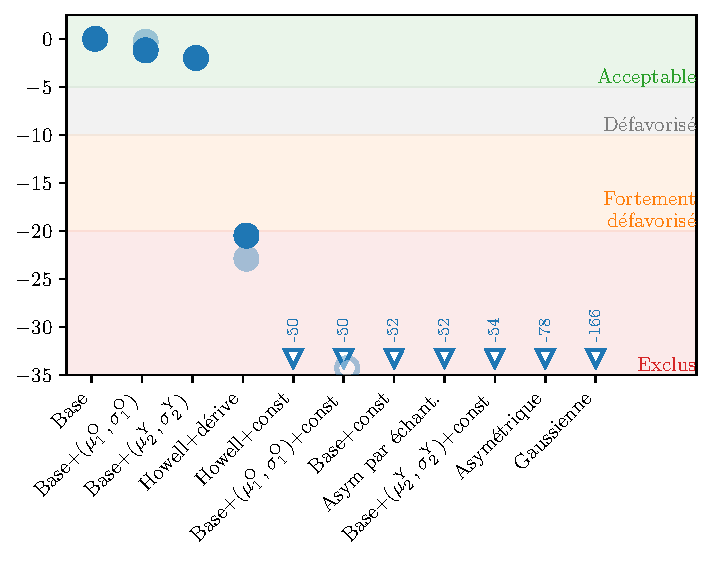
\includegraphics[width=.40\linewidth]{mod_comp_ztf-fr}
    \caption[$\Delta$AIC entre le modèle de base et les autres
    modèles]{$\Delta$AIC entre le modèle de référence et les autres modèles en
        utilisant les données de ZTF (voir Tableau~\ref{tab:comp_ztf}). La
        légende suit celle de la Figure~\ref{fig:mod_comp}. En suivant ces
        valeurs d'AIC, tous les modèles sans dérive (marqueurs ouverts) sont
        exclus car il représentent moins bien les données que le modèle de
    référence, avec dérive.}
    \label{fig:mod_comp_ztf}
\end{SCfigure}
% \sidecaptionvpos{figure}{t}

\begin{table}[p]
    \centerfloat
    \thisfloatpagestyle{empty}
    \caption[Comparaison de la capacité relative de chaque modèle à décrire les
    données par rapport au modèle de base avec les données de ZTF]{Comparaison
        de la capacité relative de chaque modèle à décrire les données en
    utilisant les données de ZTF} \label{tab:comp_ztf}
    \begin{threeparttable}
        \makebox[\linewidth]{
        \begin{tabular}{lcccccccc}
            \toprule
            & & & \multicolumn{3}{c}{Échantillon fiduciel+ZTF (1207 SNe)}
                & \multicolumn{3}{c}{Échantillon conservatif+ZTF (815 SNe)} \\
            \cmidrule(lr){4-6} \cmidrule(lr){7-9}
            Nom & dérive & $k$ &
            $-2\ln(L)$ & AIC & $\Delta$AIC & $-2\ln(L)$ & AIC & $\Delta$AIC\\
            \midrule
            % Quad. Gauss & $\delta(z)$ & 10
            % & 3344,0 & 3364,0 & 2,5 
            % & 2204,7 & 2224,7 & 8,6 \\
            Base & $\delta(z)$ & 5
            & 3348,7 & 3358,7 & -- 
            & 2215,5 & 2225,5 & -- \\
            Base+$(\mu_1^{\rm O},\sigma_1^{O})$ & $\delta(z)$ & 7
            & 3345,9 & 3359,9 & -1,2 
            & 2211,8 & 2225,8 & -0,3 \\
            Base+$(\mu_2^{\rm Y},\sigma_2^{Y})$ & $\delta(z)$ & 6
            & 3348,7 & 3360,7 & -2,0 
            & 2215,5 & 2227,5 & -2,0 \\
            Howell+dérive & $\delta(z)$ & 4
            & 3371,1 & 3379,1 & -20,5
            & 2240,4 & 2248,4 & -22,9 \\
            Howell+constant & $f$ & 5
            & 3398,3 & 3408,3 & -49,6
            & 2252,8 & 2262,8 & -37,2 \\
            Base+$(\mu_1^{\rm O},\sigma_1^{O})$+const & $f$ & 8
            & 3393,1 & 3409,1 & -50,4
            & 2243,8 & 2259,8 & -34,3 \\
            Base+const & $f$ & 6
            & 3398,3 & 3410,3 & -51,6
            & 2252,8 & 2264,8 & -39,2 \\
            Asym.\ par échant. & Par échant. & 3$\times$6
            & 3374,3 & 3410,3  & -51,7
            & 2240,9 & 2276,9  & -51,3 \\
            Base+$(\mu_2^{\rm Y},\sigma_2^{Y})$+const & $f$ & 7
            & 3398,3 & 3412,3 & -53,6
            & 2252,8 & 2266,8 & -41,2 \\
            % Quad. Gauss+const & $f$ & 11
            % & 3392,3 & 3414,3 & -55,6
            % & 2248,9 & 2270,9 & -37,6 \\
            Asymétrique & -- & 3
            & 3431,1 & 3437,1 & -78,5
            & 2278,3 & 2284,3 & -58,8 \\
            Gaussienne & -- & 2
            & 3520,5 & 3524,5 & -165,8
            & 2365,6 & 2369,6 & -144,0 \\
            \bottomrule
        \end{tabular}}
        \begin{tablenotes}[flushleft]
            \item\small \textbf{\hspace{-3.2pt}Notes.} Pour chaque modèle considéré,
                nous indiquons si le modèle dérive ou non, son nombre de
                paramètres libres $k$, et pour les échantillons fiduciel et
                conservatif, $-2\ln(L)$ (voir Équation~\ref{eq:likelihood}),
                l'AIC et la différence d'AIC ($\Delta$AIC) entre ce modèle et le
                modèle de base, choisi comme référence car présentant l'AIC le
                plus faible.
        \end{tablenotes}
    \end{threeparttable}
\end{table}
\end{landscape}
\restoregeometry

Nous voyons ici que l'incompatibilité visuelle entre HD+ZTF et N21+ZTF se
traduit très fortement au niveau de la différence d'AIC. En effet, nous
remarquons d'abord que le modèle de base s'établit encore comme le modèle de
référence. Les différentes variations au modèle de la
Section~\ref{ssec:testsupp} restent proches du modèle de base, mais toujours
défavorisés par l'AIC. En revanche, cette fois ci l'écart d'AIC avec le modèle
Howell+dérive est de 20,7, excluant cette modélisation comme bonne
représentation des données par rapport au modèle de base. L'exclusion des
modèles non-dérivants est également renforcée, le premier modèle non-dérivant
ayant un AIC 49,7 plus petit que notre modèle de référence, et 29,2 plus petit
que Howell+dérive. De manière surprenante, le modèle asymétrique pur est rendu à
l'avant-dernière place du classement étant maintenant l'une des pires
modélisations alors qu'elle était la première non-dérivante précédemment.

Bien que l'ajout de ces données donne plus de robustesse aux conclusions
principales sur la dérive de l'étirement avec le redshift, la question se pose
de la qualité de ces nouveaux paramètres pour décrire les échantillons déjà
existants. Pour cela, nous avons calculé la quantité $-2\ln(L)$ pour chacun des
modèles N21 et N21+ZTF, ajustés sur leurs échantillons respectifs, quand nous les
comparons aux données des sondages. La Figure~\ref{fig:bzcomp} et le
Tableau~\ref{tab:bzcomp} résument ces résultats.

\begin{figure}[ht]
    \centerfloat
    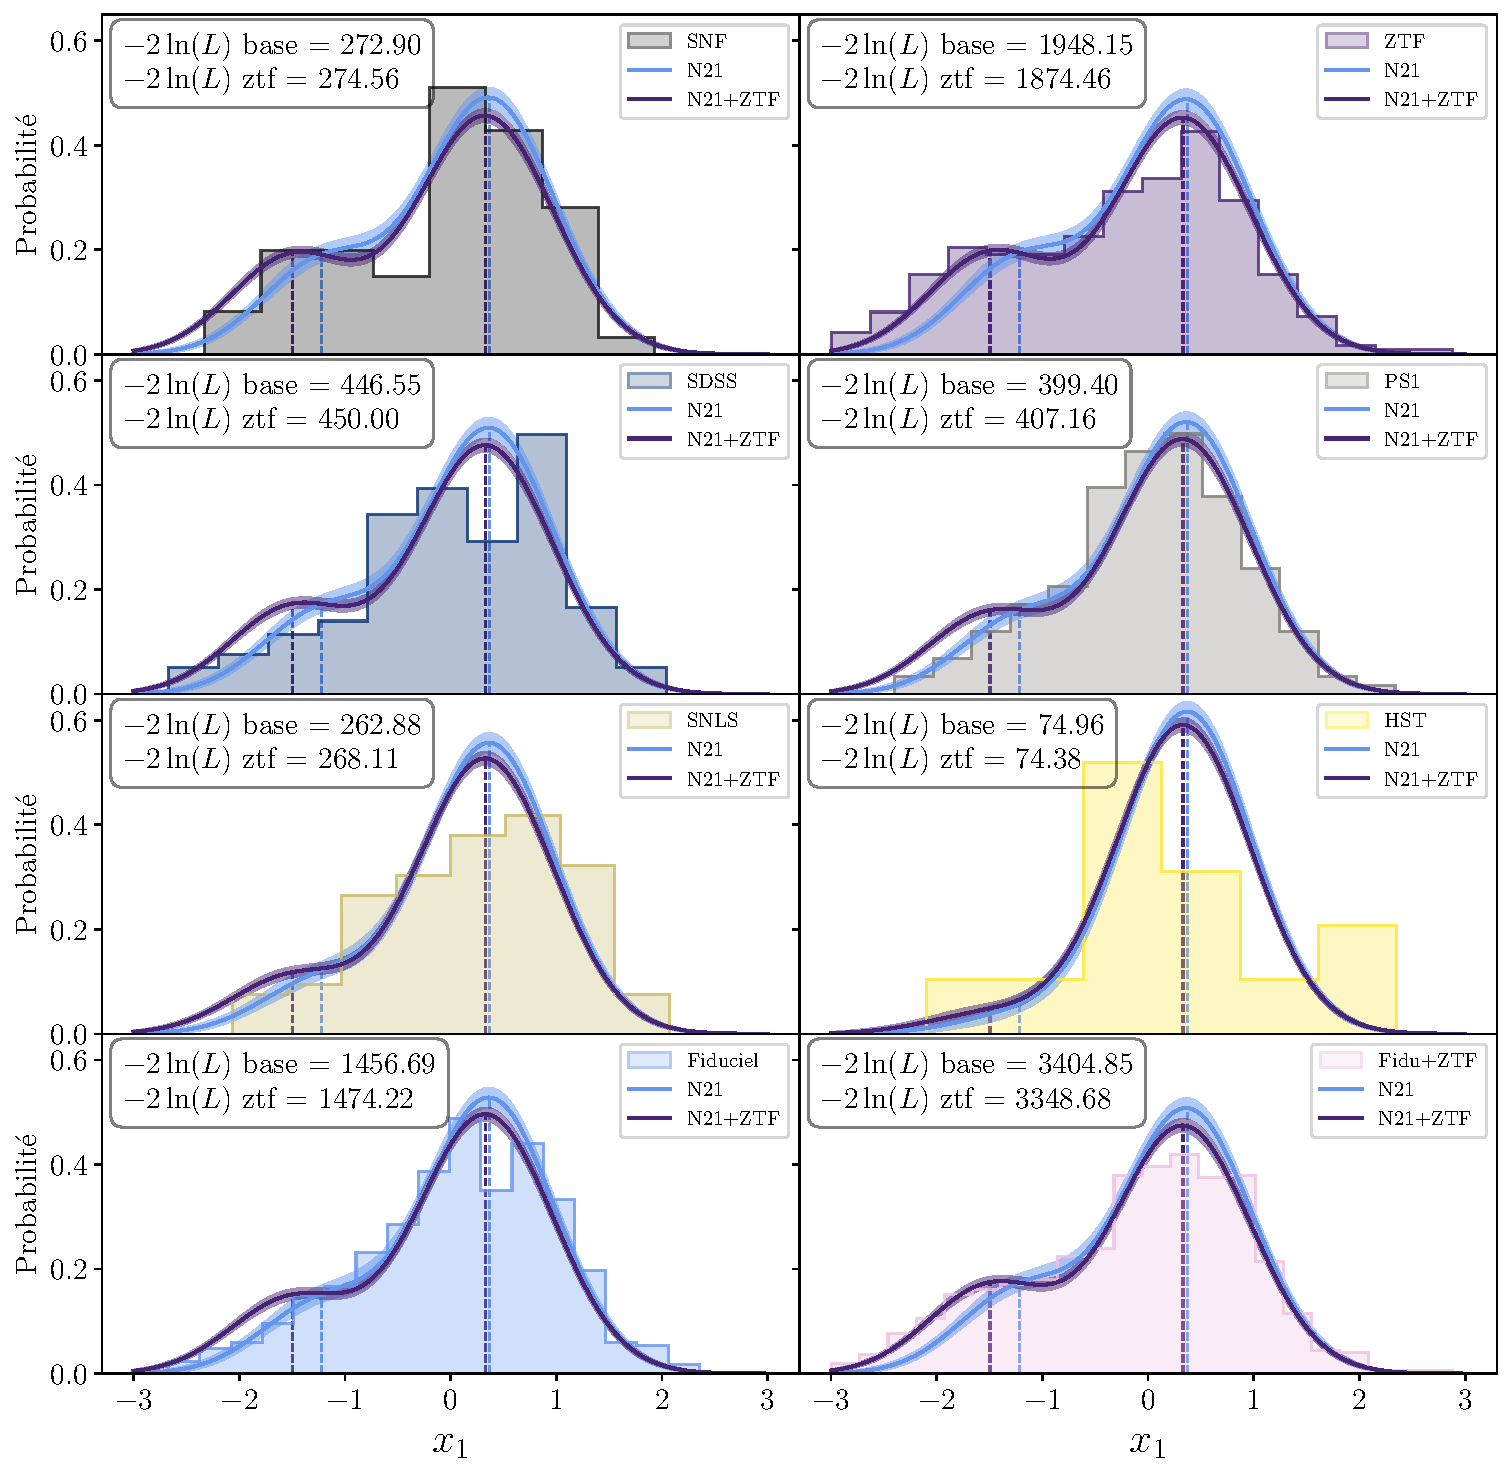
\includegraphics[width=0.8\linewidth]{model_N21+ZTF_on_allsurvs}
    \caption[Comparaison de la capacité des modèles N21 et N21+ZTF à représenter
    les données des sondages]{Comparaison de la capacité des modèles N21 et
    N21+ZTF à représenter les données des sondages. Pour chaque sondage, nous
traçons l'histogramme correspondant et les modèles N21 et N21+ZTF au redshift
moyen dudit sondage en ligne (et bande) bleue et violette respectivement (et
leurs erreurs). Le modèle N21 présente un meilleur ajustement pour chacun des
sondages sauf pour ZTF, rendant l'accord bien plus qualitatif quand ce dernier
est inclus dans l'échantillon total que quand il ne l'est pas.}
    \label{fig:bzcomp}
\end{figure}

\begin{table}[ht]
    \centering
        \caption[Capacité des modèles N21 et N21+ZTF à représenter les
        données]{Valeurs des quantités $-2\ln(L)$ des modèles N21 et N21+ZTF par
        sondage.}
        \label{tab:bzcomp}
    \begin{threeparttable}
        \makebox[\linewidth]{%
        \begin{tabular}{lcccccccc}
            \toprule
            & \multicolumn{8}{c}{Sondage}\\
            \cmidrule(lr){2-9}
            Modèle & SNF & ZTF & SDSS & PS1 & SNLS & HST & Base & Base+ZTF\\
            \midrule
            N21 &
            272,9 & 1948,2 & 446,6 & 399,4 & 262,9 & 75,0 & 1456,7 & 3404,9\\
            N21+ZTF & 
            274,6 & 1874,5 & 450,0 & 407,2 & 268,1 & 74,4 & 1474,2 & 3348,7\\
            Variation &
            1,66 & -73,69 & 3,45 & 7,76 & 5,23 & -0,57 & 17,53 & -56,16\\
            \bottomrule
    \end{tabular}}
        \begin{tablenotes}[flushleft]
        \item\small \textbf{\hspace{-3.2pt}Notes.} N21 correspond au modèle de
            base ajusté sur l'échantillon fiduciel de base. N21+ZTF correspond
            au même modèle mais ajusté sur l'échantillon fiduciel de base
            combiné à celui de ZTF.
        \end{tablenotes}
    \end{threeparttable}
\end{table}

Nous observons que le modèle N21 présente une meilleure capacité à décrire les
données que ne sont pas ZTF, avec une différence de $-2\ln(L)$ augmentant de SNf
à PS1 où nous trouvons une différence de 7,76 en faveur de N21, avant de
redescendre jusqu'à avoir une différence de -0,57 en faveur de N21+ZTF. En
revanche, chaque modèle présente une meilleure capacité à décrire son
échantillon que l'autre, comme attendu. Nous pouvons avancer que l'intégration
de ce nouvel ensemble de données, statistiquement supérieur au précédent et sur
une plage limitée de redshift, biaise la capacité du modèle à représenter les
données en lui imposant de reproduire les caractéristiques de cet échantillon
particulier.


\section{Simulations~: améliorations}\label{sec:simpersp}

Types de simulations~:
\begin{itemize}
    \item SSIZE
    \item VFULL
    \item BVSIZE~?
\end{itemize}

% Using a different tracer: simulate with age and fit with mass for the time
% being, but could extend to different tracers like local color;

% Effects of dust in the model

% Evolution of galaxies: evolution of age with redshift (K) could be freed.

% Simulation allow to test the effect of selection; upcoming surveys use galaxy
% redshit: what is the effect of selection
% Galactic selection function

\subsection{XXX}
%\label{ssec:xxx}

\subsection{XXX}
%\label{ssec:xxx}

\clearpage

\thispagestyle{plain}
% \vspace*{-3cm}
\vfill
\minilof
\vfill
\minilot
\vfill

\bibliographystyle{../main/aa_url}
\shorthandoff{:}
\bibliography{../chapters/99_references}

\end{document}
